\documentclass[11pt]{article}

\usepackage{amsmath}
\usepackage{textcomp}
\usepackage[top=0.8in, bottom=0.8in, left=0.8in, right=0.8in]{geometry}
\usepackage{listings}
\usepackage{graphicx}
\usepackage{subcaption}

% Add other packages here %



% Put your group number and names in the author field %
\title{\bf Excercise 1.\\ Implementing a first Application in RePast: A Rabbits Grass Simulation.}
\author{Group 24: Benvenuti Eloi Jean, Timothée-Florian Sébastien Bronner}

\begin{document}
\lstset{language=java}
\maketitle

\section{Implementation}

\subsection{Assumptions}
% Describe the assumptions of your world model and implementation (e.g. is the grass amount bounded in each cell) %
The world is a 2D grid of with no border on the edge (it's a torus). On this world there are rabbits and grass. The rabbits move randomly on one of the fourth cardinal directions and eat the grass under then if any. The grass growth randomly (independently of the rabbits' position) at each step. The grass can growth under a rabbit.

When a rabbit eats grass, its internal energy grows. At each step this internal energy is also decreased to simulate the rabbit's metabolism needs. If the rabbit has no energy left, it dies. If its energy reaches a certain threshold, it reproduces.

When a rabbit reproduces, it has to pay a certain amount of energy and its child is put somewhere on the world, if there is enough room left.

\subsection{Implementation Remarks}
% Provide important details about your implementation, such as handling of boundary conditions %
\paragraph{World is a torus} In order to make the world "loop around" we use the following piece of code.
\begin{lstlisting}[frame=single]
  newX = (newX + grid.getSizeX())%grid.getSizeX();
  newY = (newY + grid.getSizeY())%grid.getSizeY();
\end{lstlisting}

%what we do if there is no room left on the gird
\paragraph{No room left on the grid}One of the bug we ran into was that the program would throw an error if the grid was filled with rabbits and a new rabbit was created. This was because the rabbit we added to a list of existing agents but wasn't added on the grid. So we wrote an if-statement that prevent new rabbits from being born if the gird is full.

%How the rabbit move
\paragraph{Movement protocol of the rabbits} The rabbits can only move following one of the fourth cardinal directions. It cannot move on an already occupied case. The decision process of the rabbit goes as follow.

\begin{enumerate}
  \item Randomly picks one of the 4 directions.
  \item Checks if the case is free.
  \item If yes, moves on it, otherwise stays put.
\end{enumerate}

%Condition of death and energy depletion
\paragraph{Energy management} Each rabbit, be it created at the start of the simulation or later by reproduction, starts with a set amount of energy, defined by the user (AgentEnergyAtBirth). At each step the rabbit will lose 1 energy. It will also gain energy by consumming the grass present at its possition after its movement phase.%if there is some grass on his tile because he will eat it, thus destroying the grass.

If the energy of a rabbit goes over the reproduction threshold, which can be set by the user(AgentReproductionThreshold), he immediately reproduces by paying a cost equal to the one specified in the user-settable variable (AgentReproductionCost). Paying this cost can kill him and even set its energy way below 0 (see section \ref{sec:experiment3}).

Finally, if and only if the rabbit's energy drops below 1, he dies. 

%About the grass
\paragraph{The grass} The grass growth can be set by the user with the variable GrassGrowth. If the variable is equal to 1000, for example, it means that 1000 units of grass, each containing 1 energy, will appear randomly independently of the rabbits's position. There can be multiple units of grass on one tile, thus increasing the energy value of the tile. When a rabbit steps on it, all the grass is consumed.

\section{Results}
% In this section, you study and describe how different variables (e.g. birth threshold, grass growth rate etc.) or combinations of variables influence the results. Different experiments with different settings are described below with your observations and analysis

\subsection{Experiment 1}

\subsubsection{Setting}
The variables were set to the following values:
\begin{lstlisting}
  Energy at birth: 20
  Reproduction cost: 30
  Reproduction Threshold 50
  Grass growth:1000
  Num Agents: 100
  World: 100x100
\end{lstlisting}
\subsubsection{Observations}
% Elaborate on the observed results %
We observe a rapid growth at the beginning of the simulation (Figures \ref{img:rabbits1} and \ref{img:grass1}), both for the number of rabbits and the quantity of grass on the world. Then both populations stabilize around 1000 rabbits and 15000 units of grass, respectively. We suppose that the intial surge is due to the fact that the grid was relatively empty at the beginning (only 100 rabbits and 1000 grass) so there was a growth spike before the agents had to compete for resources.
\begin{figure}
    \begin{tabular}{c c c}
         \begin{subfigure}[b]{0.3\textwidth}
        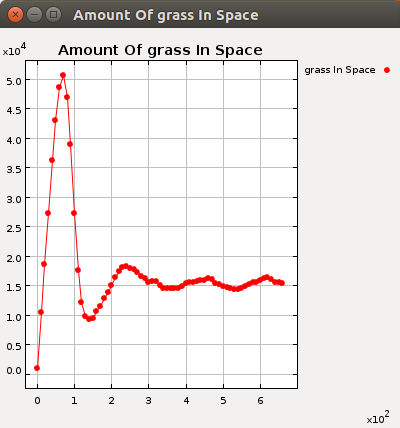
\includegraphics[width=\textwidth]{experiment/1/Grass.png}
        \caption{\label{img:grass1} Grass level for experiment 1}
    \end{subfigure} & 
    \begin{subfigure}[b]{0.3\textwidth}
        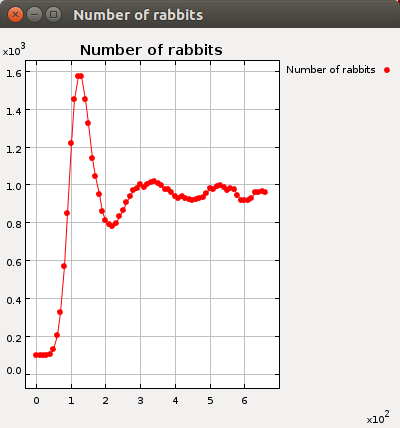
\includegraphics[width=\textwidth]{experiment/1/Rabbits.png}
        \caption{\label{img:rabbits1} Rabbits level for experiment 1}
    \end{subfigure} &
    \begin{subfigure}[b]{0.3\textwidth}
        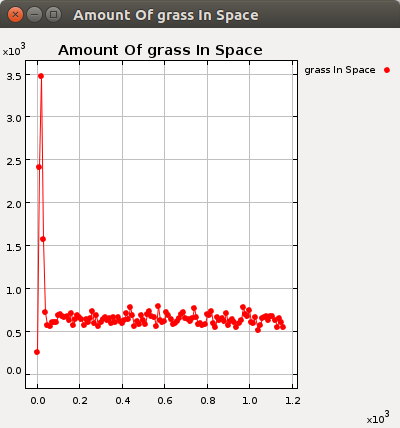
\includegraphics[width=\textwidth]{experiment/2/Grass.png}
        \caption{\label{img:grass2} Grass level for experiment 2}
    \end{subfigure}\\
    \begin{subfigure}[b]{0.3\textwidth}
        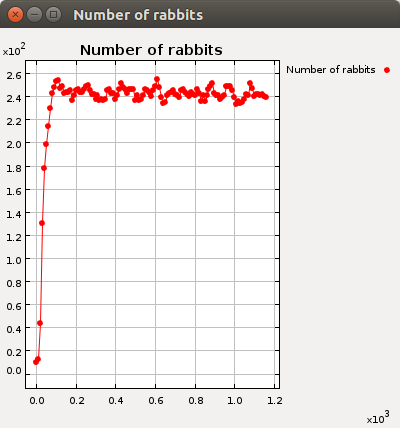
\includegraphics[width=\textwidth]{experiment/2/Rabbits.png}
        \caption{\label{img:rabbits2} Rabbits level for experiment 2}
    \end{subfigure} & 
    \begin{subfigure}[b]{0.3\textwidth}
        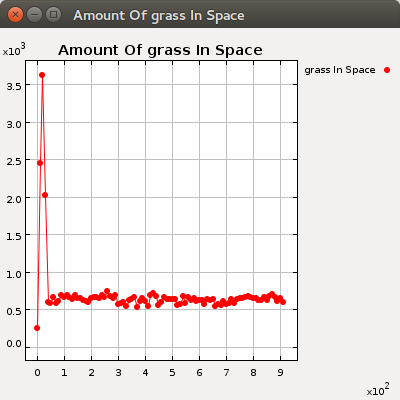
\includegraphics[width=\textwidth]{experiment/3/Grass.png}
        \caption{\label{img:grass3} Grass level for experiment 3}
    \end{subfigure} &
    \begin{subfigure}[b]{0.3\textwidth}
        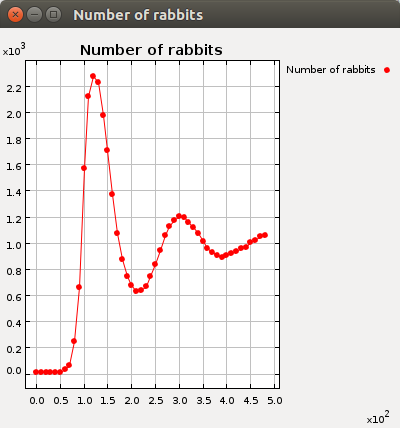
\includegraphics[width=\textwidth]{experiment/3/Rabbits.png}
        \caption{\label{img:rabbits3} Rabbits level for experiment 3}
    \end{subfigure}
   
    \end{tabular}
  \caption{Grass and rabbits level for the three experiments.}
\end{figure}

\subsection{Experiment 2}

\subsubsection{Setting}

\subsubsection{Observations}
% Elaborate on the observed results %

\subsection{Experiment 3}
\label{sec:experiment3}

\subsubsection{Setting}

\subsubsection{Observations}
% Elaborate on the observed results %

\end{document}
